\documentclass[a4paper,12pt]{article}

% Packages
\usepackage[utf8]{inputenc}
\usepackage[T1]{fontenc}
\usepackage[french]{babel}
\usepackage{amsmath}
\usepackage{amssymb}
\usepackage{graphicx}
\usepackage{float}
\usepackage{geometry}

% Marges
\geometry{margin=2.5cm}

% Informations du document
\title{Filtre de Kalman}
\author{Fatimetou Narjah}
\date{Octobre 2026}

\begin{document}

\maketitle

\section{Question 1 -- Localisation GNSS avec un filtre de Kalman}

Dans cette partie, on applique un filtre de Kalman à un problème
simplifié de localisation GNSS. Le vecteur d'état est composé de la
position et de la vitesse du système :

\begin{equation}
X_k =
\begin{bmatrix}
\mathrm{Pos}_k\\
\mathrm{Vel}_k
\end{bmatrix}
\in \mathbb{R}^6.
\end{equation}

Le modèle d'évolution utilisé est, pour $\Delta t = 1$ :

\begin{equation}
X_k =
\begin{bmatrix}
I_3 & \Delta t I_3\\
0_3 & I_3
\end{bmatrix}
X_{k-1} + \eta_k,
\qquad
\eta_k \sim \mathcal{N}(0,Q).
\end{equation}

Le modèle d'observation est :

\begin{equation}
Y_k =
\begin{bmatrix}
I_3 & 0_3
\end{bmatrix}
X_k + \nu_k,
\qquad
\nu_k \sim \mathcal{N}(0,R).
\end{equation}

Ainsi, les mesures GNSS fournissent directement une information sur
la position, tandis que la vitesse est estimée par le filtre à partir
du modèle dynamique et des mesures successives.


\subsection{1.a -- Implémentation du filtre de Kalman}

Le filtre de Kalman fonctionne en deux étapes principales : la
prédiction et la correction.

Lors de la prédiction, l'état précédent est propagé à l'instant
suivant à l'aide du modèle dynamique :

\begin{equation}
X_{k|k-1} = F X_{k-1|k-1},
\end{equation}

avec

\begin{equation}
F =
\begin{bmatrix}
I_3 & \Delta t I_3\\
0_3 & I_3
\end{bmatrix}.
\end{equation}

La covariance prédite est donnée par :

\begin{equation}
P_{k|k-1}
=
F P_{k-1|k-1} F^T + Q.
\end{equation}

Lorsque la mesure GNSS $Y_k$ est disponible, le filtre calcule
l'innovation :

\begin{equation}
\widetilde{Y}_k
=
Y_k-HX_{k|k-1},
\end{equation}

avec

\begin{equation}
H =
\begin{bmatrix}
I_3 & 0_3
\end{bmatrix}.
\end{equation}

La covariance de l'innovation est :

\begin{equation}
S_k =
HP_{k|k-1}H^T+R.
\end{equation}

Le gain de Kalman est alors calculé par :

\begin{equation}
K_k =
P_{k|k-1}H^T
\left(
HP_{k|k-1}H^T+R
\right)^{-1}.
\end{equation}

L'état est ensuite corrigé à partir de la mesure :

\begin{equation}
X_{k|k}
=
X_{k|k-1}
+
K_k
\left(
Y_k-HX_{k|k-1}
\right).
\end{equation}

Enfin, la covariance après correction est donnée par :

\begin{equation}
P_{k|k}
=
(I-K_kH)P_{k|k-1}.
\end{equation}

La figure suivante présente les résultats obtenus avec le filtre de
Kalman dans le cas nominal.


\begin{figure}
        \centering
        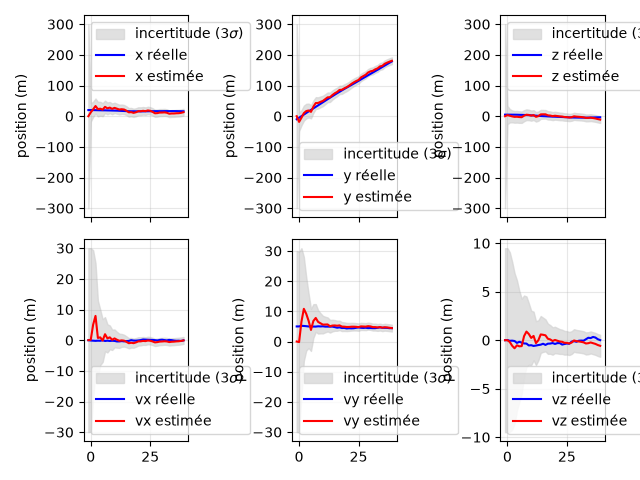
\includegraphics[width=0.95\linewidth]{Q1.png}
        \caption{Résultats du filtre de Kalman dans le cas nominal :
    positions et vitesses réelles et estimées, avec l'incertitude
    représentée par $3\sigma$.}
    \label{fig:q1_reference}
\end{figure}

On observe que les estimations des positions suivent correctement les
valeurs réelles. Les courbes estimées restent proches des courbes réelles,
ce qui montre que le filtre combine efficacement les prédictions du modèle
dynamique et les mesures GNSS.

Les trois composantes de la vitesse ne sont pas directement mesurées par
le modèle d'observation. Elles sont donc estimées indirectement à partir
du modèle dynamique et de l'évolution successive des positions.

Au début de la simulation, l'incertitude est relativement importante en
raison de l'incertitude initiale sur l'état. Lorsque les mesures GNSS sont
disponibles, l'étape de correction permet de réduire la covariance de
l'estimation. Entre deux mesures, la covariance peut cependant augmenter
à nouveau lors de la prédiction à cause du terme $Q$.

La zone grise représente l'intervalle d'incertitude correspondant à
$\pm3\sigma$. On constate ainsi que le filtre devient progressivement plus
confiant dans son estimation lorsque les observations sont régulièrement
disponibles.


\subsection{1.b -- Trou de mesure}

Pour cette expérience, les mesures GNSS sont volontairement
supprimées pendant un intervalle de temps, par exemple entre
$t=10$ et $t=20$.

Pendant cette période, aucune nouvelle mesure de position n'est
disponible pour le filtre. L'étape de correction ne peut donc pas être
effectuée. Le filtre réalise uniquement l'étape de prédiction :

\begin{equation}
X_{k|k}=X_{k|k-1},
\end{equation}

et la covariance continue d'être propagée selon :

\begin{equation}
P_{k|k-1}
=
FP_{k-1|k-1}F^T+Q.
\end{equation}

La figure suivante montre le comportement du filtre pendant le trou
de mesure.

\begin{figure}[H]
    \centering
    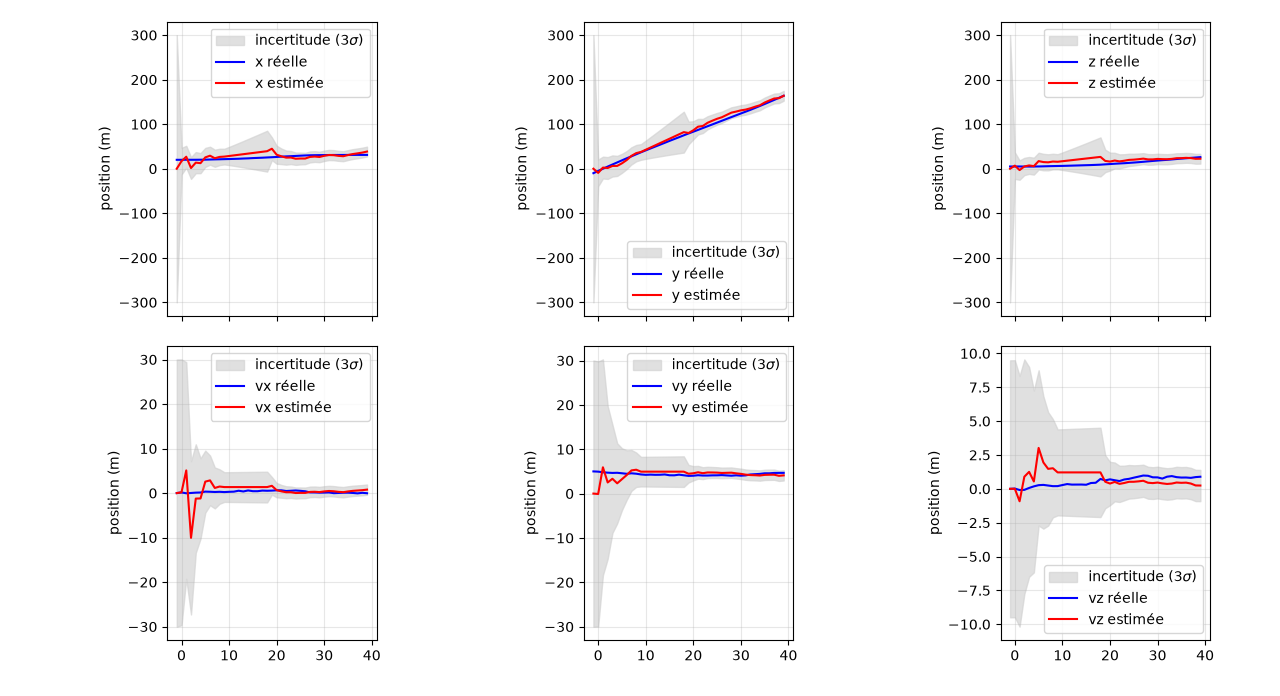
\includegraphics[width=0.95\textwidth]{Q1_trou_mesure.png}
    \caption{Comportement du filtre lors du trou de mesure GNSS entre
    $t=10$ et $t=20$.}
    \label{fig:q1_trou}
\end{figure}

On observe que, pendant le trou de mesure, l'incertitude augmente
progressivement. En effet, à chaque étape de prédiction, le terme $Q$
est ajouté à la covariance. Comme aucune mesure n'est disponible,
aucune étape de correction ne vient réduire cette covariance.

L'erreur d'estimation peut également augmenter pendant cette période.
Le filtre continue à faire évoluer l'état uniquement à partir du
modèle dynamique. Les erreurs du modèle et le bruit de dynamique
s'accumulent donc progressivement.

Lorsque les mesures GNSS redeviennent disponibles, le filtre reprend
l'étape de correction. Les nouvelles mesures permettent alors de
corriger l'estimation et de réduire progressivement l'incertitude.

Cette expérience montre donc l'importance des mesures : même si le
filtre peut continuer à fonctionner en l'absence temporaire de
mesures, son incertitude augmente tant qu'aucune observation ne permet
de corriger la prédiction.


\subsection{1.c -- Influence du bruit de dynamique $Q$}

Dans cette expérience, nous étudions l'influence de la matrice $Q$,
qui représente le bruit associé au modèle dynamique. La covariance
prédite est donnée par :

\begin{equation}
P_{k|k-1}=F P_{k-1|k-1}F^T+Q.
\end{equation}

Initialement,

\begin{equation}
Q_{\mathrm{initial}}
=
\operatorname{diag}
(10^{-4},10^{-4},10^{-4},10^{-2},10^{-2},10^{-2}).
\end{equation}

Nous avons ensuite augmenté $Q$ d'un facteur $100$ :

\begin{equation}
Q_{\mathrm{nouveau}}=100Q_{\mathrm{initial}}
=
\operatorname{diag}(10^{-2},10^{-2},10^{-2},1,1,1).
\end{equation}

\begin{figure}[H]
    \centering
    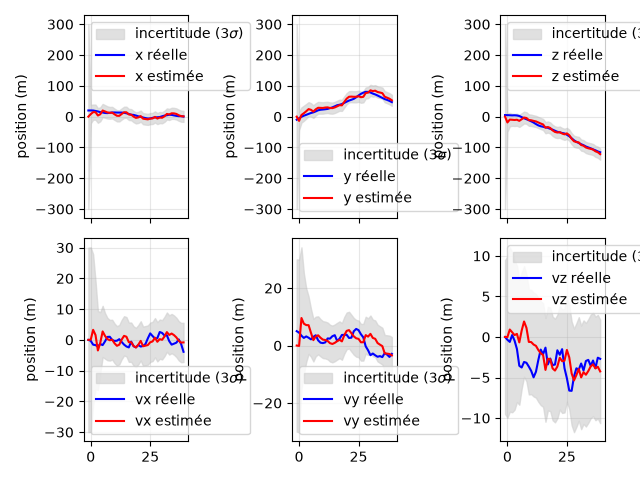
\includegraphics[width=0.95\textwidth]{Q1_variation_Q.png}
    \caption{Influence de l'augmentation du bruit de dynamique $Q$.}
    \label{fig:q1_Q}
\end{figure}

On observe que l'augmentation de $Q$ élargit les bandes d'incertitude,
car la covariance prédite augmente :

\[
Q\uparrow
\quad\Longrightarrow\quad
P_{k|k-1}\uparrow
\quad\Longrightarrow\quad
\sigma\uparrow.
\]

L'effet est particulièrement visible sur les vitesses $v_x$, $v_y$ et
$v_z$. En effet, les mesures GNSS observent directement la position
mais pas la vitesse :

\begin{equation}
H=
\begin{bmatrix}
I_3 & 0_3
\end{bmatrix}.
\end{equation}

Les positions sont donc régulièrement corrigées par les mesures, tandis
que les vitesses sont estimées indirectement à partir du modèle dynamique.
Elles sont ainsi plus sensibles à l'augmentation du bruit de processus
$Q$. L'information de position permet néanmoins de corriger indirectement
les vitesses grâce au couplage entre position et vitesse dans la matrice
$F$.


\subsection{1.d -- Influence du bruit de mesure $R$}

Dans cette expérience, on fait varier la matrice $R$, qui représente
le bruit associé aux mesures GNSS.

La covariance de l'innovation est donnée par :

\begin{equation}
S_k = HP_{k|k-1}H^T+R.
\end{equation}

Le gain de Kalman est :

\begin{equation}
K_k =
P_{k|k-1}H^T
\left(HP_{k|k-1}H^T+R\right)^{-1}.
\end{equation}

Lorsque $R$ augmente, $S_k$ augmente et le gain de Kalman $K_k$ diminue.
Le filtre accorde donc moins de confiance aux mesures GNSS et davantage
à la prédiction issue du modèle dynamique.

\begin{figure}[H]
    \centering
    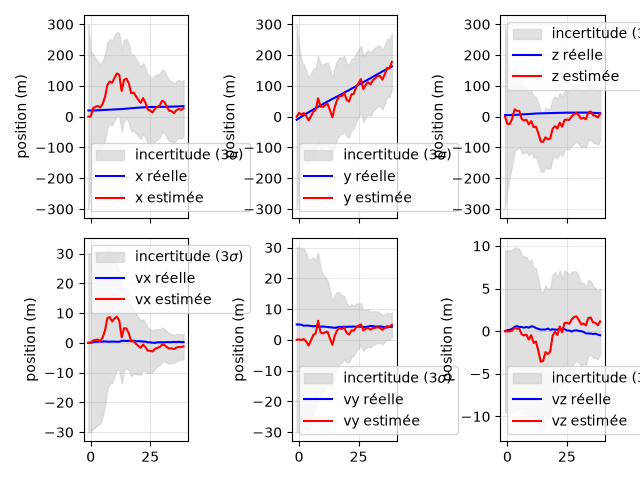
\includegraphics[width=0.95\textwidth]{Q1_variation_R.png}
    \caption{Influence de la variation du bruit de mesure $R$ sur
    l'estimation et l'incertitude du filtre.}
    \label{fig:q1_R}
\end{figure}

On observe que l'augmentation de $R$ entraîne une augmentation des bandes
d'incertitude, à la fois pour les positions et pour les vitesses. En effet,
la covariance après correction est moins réduite lorsque le gain de Kalman
diminue :

\begin{equation}
P_{k|k}=(I-K_kH)P_{k|k-1}.
\end{equation}

Les positions sont directement mesurées par le GNSS, mais lorsque $R$ est
grand, ces mesures sont considérées comme peu fiables et corrigent moins
efficacement la prédiction. La position reste donc plus incertaine.

Les vitesses ne sont pas mesurées directement. Elles dépendent de
l'information de position pour être corrigées indirectement. Lorsque les
mesures de position deviennent moins fiables à cause de l'augmentation de
$R$, cette correction indirecte des vitesses devient également moins
efficace. L'incertitude augmente donc aussi pour $v_x$, $v_y$ et $v_z$.

Ainsi, contrairement à $Q$, qui augmente directement l'incertitude lors de
la prédiction, une augmentation de $R$ réduit l'efficacité de l'étape de
correction. Dans les deux cas, l'incertitude finale du filtre augmente,
mais pour des raisons différentes.

\section{Question 2}

\subsection{Question 2.2 -- Sensor failure}

Pour étudier l'effet d'une défaillance du capteur, on modifie la fonction
\texttt{get\_observation(k)} afin qu'elle retourne \texttt{None} pendant
l'intervalle $2500 < k < 3500$ :

\begin{verbatim}
if k > 2500 and k < 3500:
    return [None, None]
\end{verbatim}

Pendant cette période, aucune observation des landmarks n'est disponible.
Le filtre effectue donc uniquement l'étape de prédiction :

\begin{verbatim}
xEst = xPred
PEst = PPred
\end{verbatim}

Ainsi,

\[
x_{k|k}=x_{k|k-1},
\]

et la covariance est propagée selon :

\[
P_{k|k-1}
=
A P_{k-1|k-1} A^T + BQB^T.
\]

\begin{figure}[H]
    \centering
    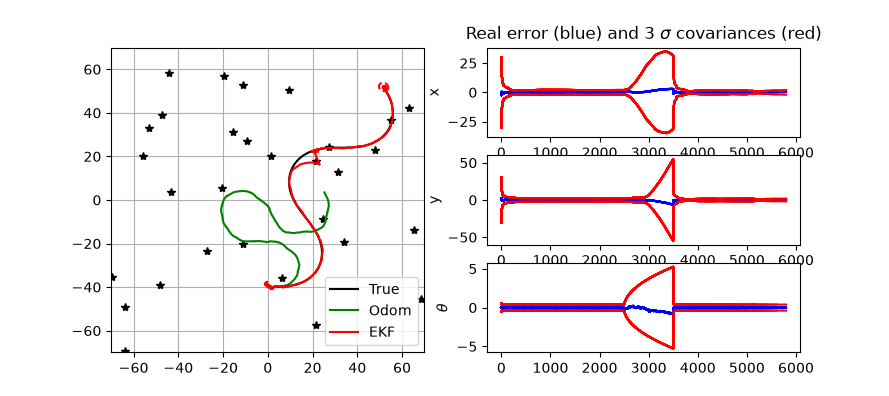
\includegraphics[width=0.9\textwidth]{Q2_apres_exclusion.png}
    \caption{Effet de la défaillance du capteur entre $k=2500$ et
    $k=3500$.}
    \label{fig:sensor_failure}
\end{figure}

Avant $k=2500$, les observations permettent au filtre de corriger
régulièrement son estimation. Entre $k=2500$ et $k=3500$, l'absence de
mesures empêche toute correction. Les erreurs de prédiction s'accumulent
et les bandes d'incertitude $3\sigma$ augmentent progressivement.

À partir de $k=3500$, les observations redeviennent disponibles. Le filtre
reprend alors l'étape de correction, ce qui permet de réduire
l'incertitude et de rapprocher progressivement l'estimation de la
trajectoire réelle.

Cette expérience montre donc que, sans observation, le filtre peut
continuer à prédire l'état grâce au modèle dynamique, mais son incertitude
augmente jusqu'au retour des mesures.

\subsection{Question 3 -- Model errors}

Dans cette question, on étudie l'influence d'une mauvaise estimation des
bruits utilisés par le filtre. Les matrices $Q_{\mathrm{True}}$ et
$P_Y^{\mathrm{True}}$ correspondent aux bruits réellement utilisés dans
le simulateur, tandis que $Q_{\mathrm{Est}}$ et $P_Y^{\mathrm{Est}}$
sont ceux supposés par le filtre.

Lorsque le bruit d'odométrie est fortement surestimé et que le bruit des
observations est sous-estimé, on utilise par exemple :

\[
Q_{\mathrm{Est}} = 100Q_{\mathrm{True}},
\qquad
P_Y^{\mathrm{Est}} = 0.1P_Y^{\mathrm{True}}.
\]

Le filtre considère alors que l'odométrie est très bruitée et accorde
donc moins de confiance à la prédiction. À l'inverse, il considère les
observations comme très précises et leur donne davantage de poids lors
de la correction.

\begin{figure}[H]
    \centering
    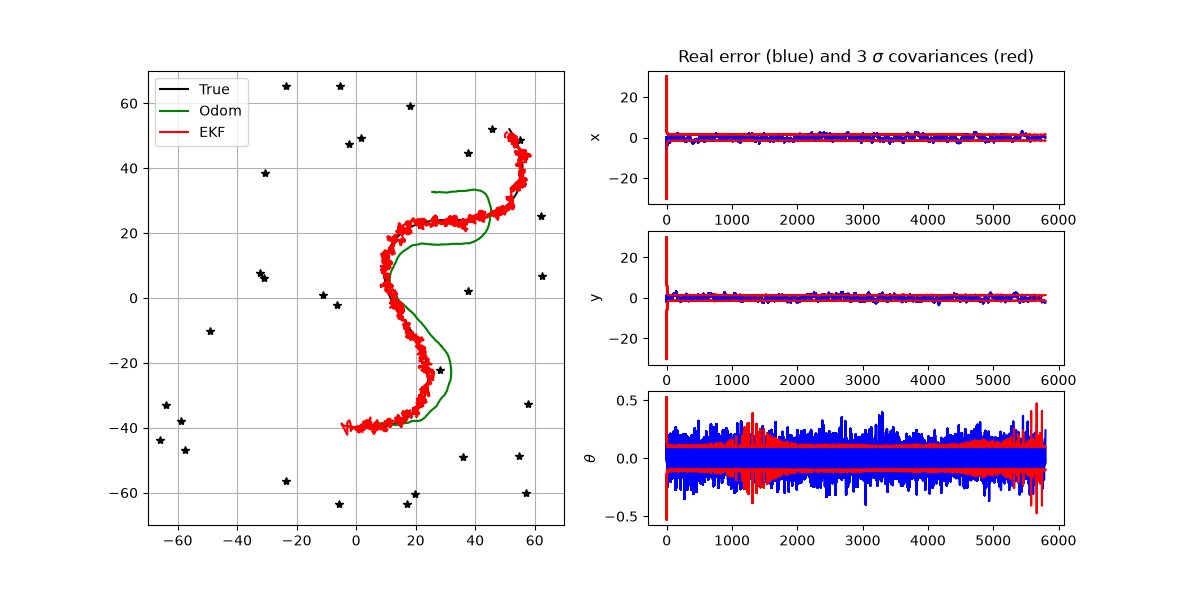
\includegraphics[width=0.95\linewidth]{Q3_Pdiminue_Qaugmente.png}
    \caption{Influence d'une forte surestimation du bruit d'odométrie et
    d'une sous-estimation du bruit des observations.}
    \label{fig:placeholder}
\end{figure}

On observe que l'estimation reste globalement proche de la trajectoire
réelle. Cependant, les erreurs et les incertitudes sont particulièrement
visibles sur l'orientation $\theta$. Cette situation montre que le filtre
fait fortement confiance aux observations pour corriger la prédiction,
car le bruit de mesure utilisé par le filtre est considéré comme faible.

Nous considérons ensuite le cas demandé dans l'énoncé où le bruit estimé
sur la distance des landmarks est important, tandis que le bruit sur
leur direction reste correct. On utilise :

\[
P_Y^{\mathrm{Est}}
=
\operatorname{diag}
\left(
100^2,
\left(\frac{6\pi}{180}\right)^2
\right).
\]

Le filtre considère alors les mesures de distance comme peu fiables et
leur attribue un poids plus faible. En revanche, les mesures de direction
restent considérées comme fiables et conservent une influence importante
dans la correction.

\begin{figure}[H]
    \centering
    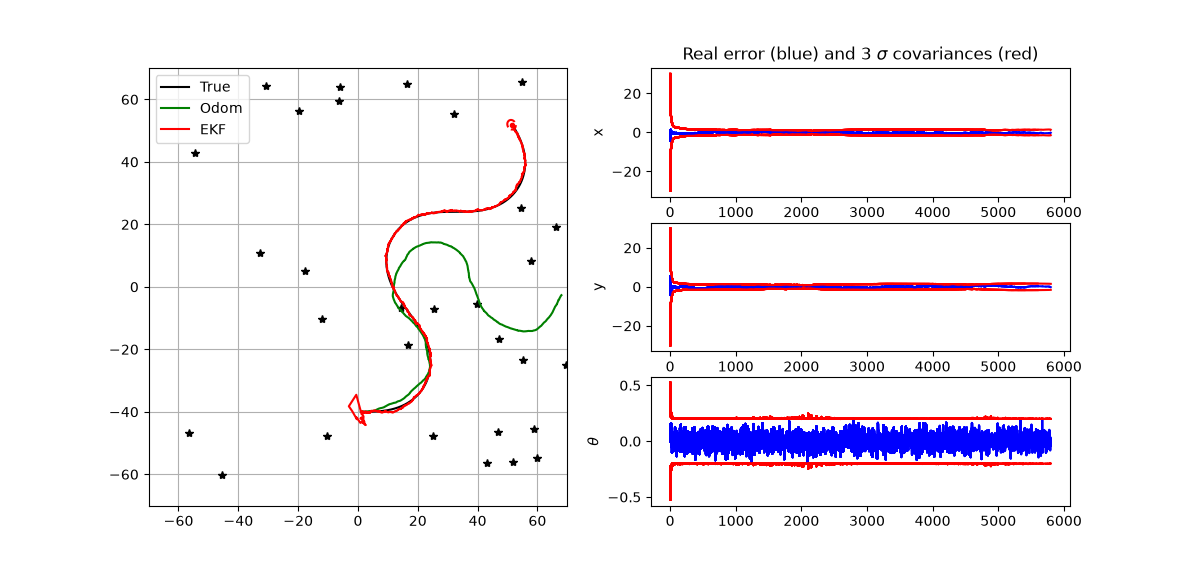
\includegraphics[width=0.95\textwidth]{Q3_distance_large_direction_correct.png}
    \caption{Estimation lorsque le bruit estimé sur la distance des
    landmarks est important tandis que le bruit sur leur direction reste
    correct.}
    \label{fig:q3_distance_large}
\end{figure}

On observe que la trajectoire estimée reste proche de la trajectoire
réelle malgré la forte incertitude sur les distances. Les informations
angulaires permettent en effet de continuer à corriger l'estimation,
notamment l'orientation. La distance n'est pas supprimée de
l'observation, mais son influence dans la correction est fortement
réduite.

Ainsi, une mauvaise estimation des matrices de covariance modifie
directement le compromis entre la prédiction et les observations. Le
filtre accorde plus ou moins de confiance à chaque source d'information
en fonction des valeurs de $Q_{\mathrm{Est}}$ et
$P_Y^{\mathrm{Est}}$.



\subsection{Question 2.4 -- Observabilité partielle}

Dans cette expérience, on étudie le comportement de l'EKF lorsque
seule une partie de l'observation des landmarks est disponible.
On considère successivement le cas où seule la distance est utilisée,
puis celui où seule la direction est utilisée.

\begin{figure}[H]
    \centering
    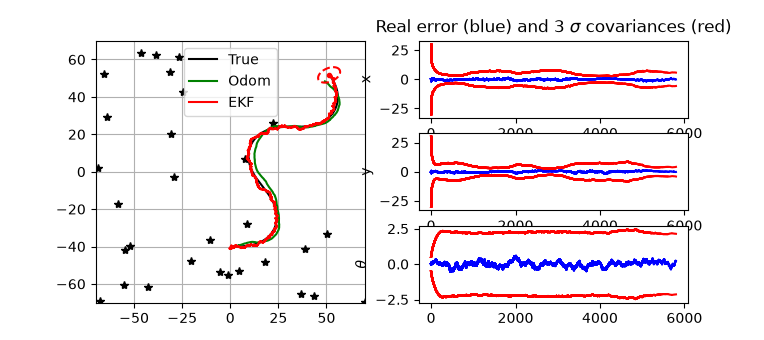
\includegraphics[width=0.95\textwidth]{Q4_distance.png}
    \caption{Estimation avec uniquement la distance aux landmarks.}
    \label{fig:q4_distance}
\end{figure}

Lorsque seule la distance est utilisée, l'observation est donnée par :

\[
z = r =
\sqrt{(x_L-x)^2+(y_L-y)^2}.
\]

La distance fournit une information sur la position du robot par rapport
aux landmarks, mais elle ne dépend pas directement de son orientation
$\theta$. Sur la figure, on observe néanmoins que l'estimation de la
trajectoire reste proche de la trajectoire réelle et que les erreurs sur
$x$ et $y$ restent faibles.

En revanche, l'incertitude sur $\theta$ est plus importante. L'orientation
est donc moins directement observable avec la distance seule et doit être
estimée en partie grâce au modèle dynamique et aux observations
successives.

\begin{figure}[H]
    \centering
    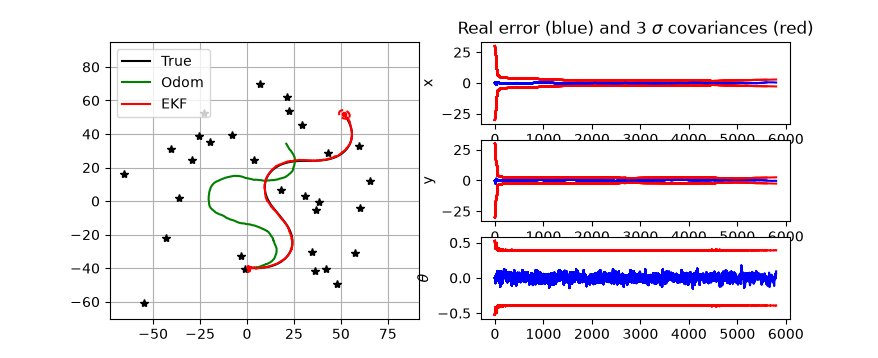
\includegraphics[width=0.95\textwidth]{Q4_direction.png}
    \caption{Estimation avec uniquement la direction des landmarks.}
    \label{fig:q4_direction}
\end{figure}

Dans le second cas, seule la direction du landmark est utilisée :

\[
z = \theta_L-\theta.
\]

Cette observation contient directement une information sur l'orientation
du robot. La figure montre que la trajectoire estimée reste également
proche de la trajectoire réelle et que les erreurs sur $x$ et $y$ restent
faibles.

L'effet est particulièrement visible sur $\theta$ : la bande
d'incertitude $3\sigma$ est nettement plus faible que dans le cas de la
distance seule. L'orientation est donc mieux contrainte lorsque la
direction du landmark est mesurée directement.

Ainsi, la distance et la direction fournissent des informations
complémentaires : la distance contraint principalement la position,
tandis que la direction apporte davantage d'information sur
l'orientation. Dans les deux cas, l'EKF reste capable de suivre la
trajectoire, mais avec une incertitude différente selon la composante
observée.


\end{document}